%%%%                          %%%%
%%%% FUNDAMENTOS TECNOLÓGICOS %%%%
%%%%                          %%%%

\chapter{Fundamentos tecnológicos}
\label{chap:fundamentos-tecnologicos}

\section{¿El formato PDF? Estructura de un PDF}

Son tres las tecnologías base que componen el formato PDF:

\begin{itemize}
	\item Los PDF se escriben como un subconjunto del lenguaje de programación PostScript.
	\item Un sistema para incrustar y reemplazar fuentes tipográficas.
	\item Un sistema estructurado de almacenamiento para unir todos los elementos en un único fichero.
\end{itemize}

Otros elementos deben incluirse en formato \acrfull{cos}. Un árbol cos contiene objetos de los siguientes tipos:

\begin{enumerate}
	\item Boolean values
	\item Numbers
	\item Strings
	\item Arrays
	\item Dictionaries
	\item Streams
	\item Null object
\end{enumerate}

Relaciones entre los espacios de coordenadas de un PDF:

\begin{figure}[hp!]
	\centering
	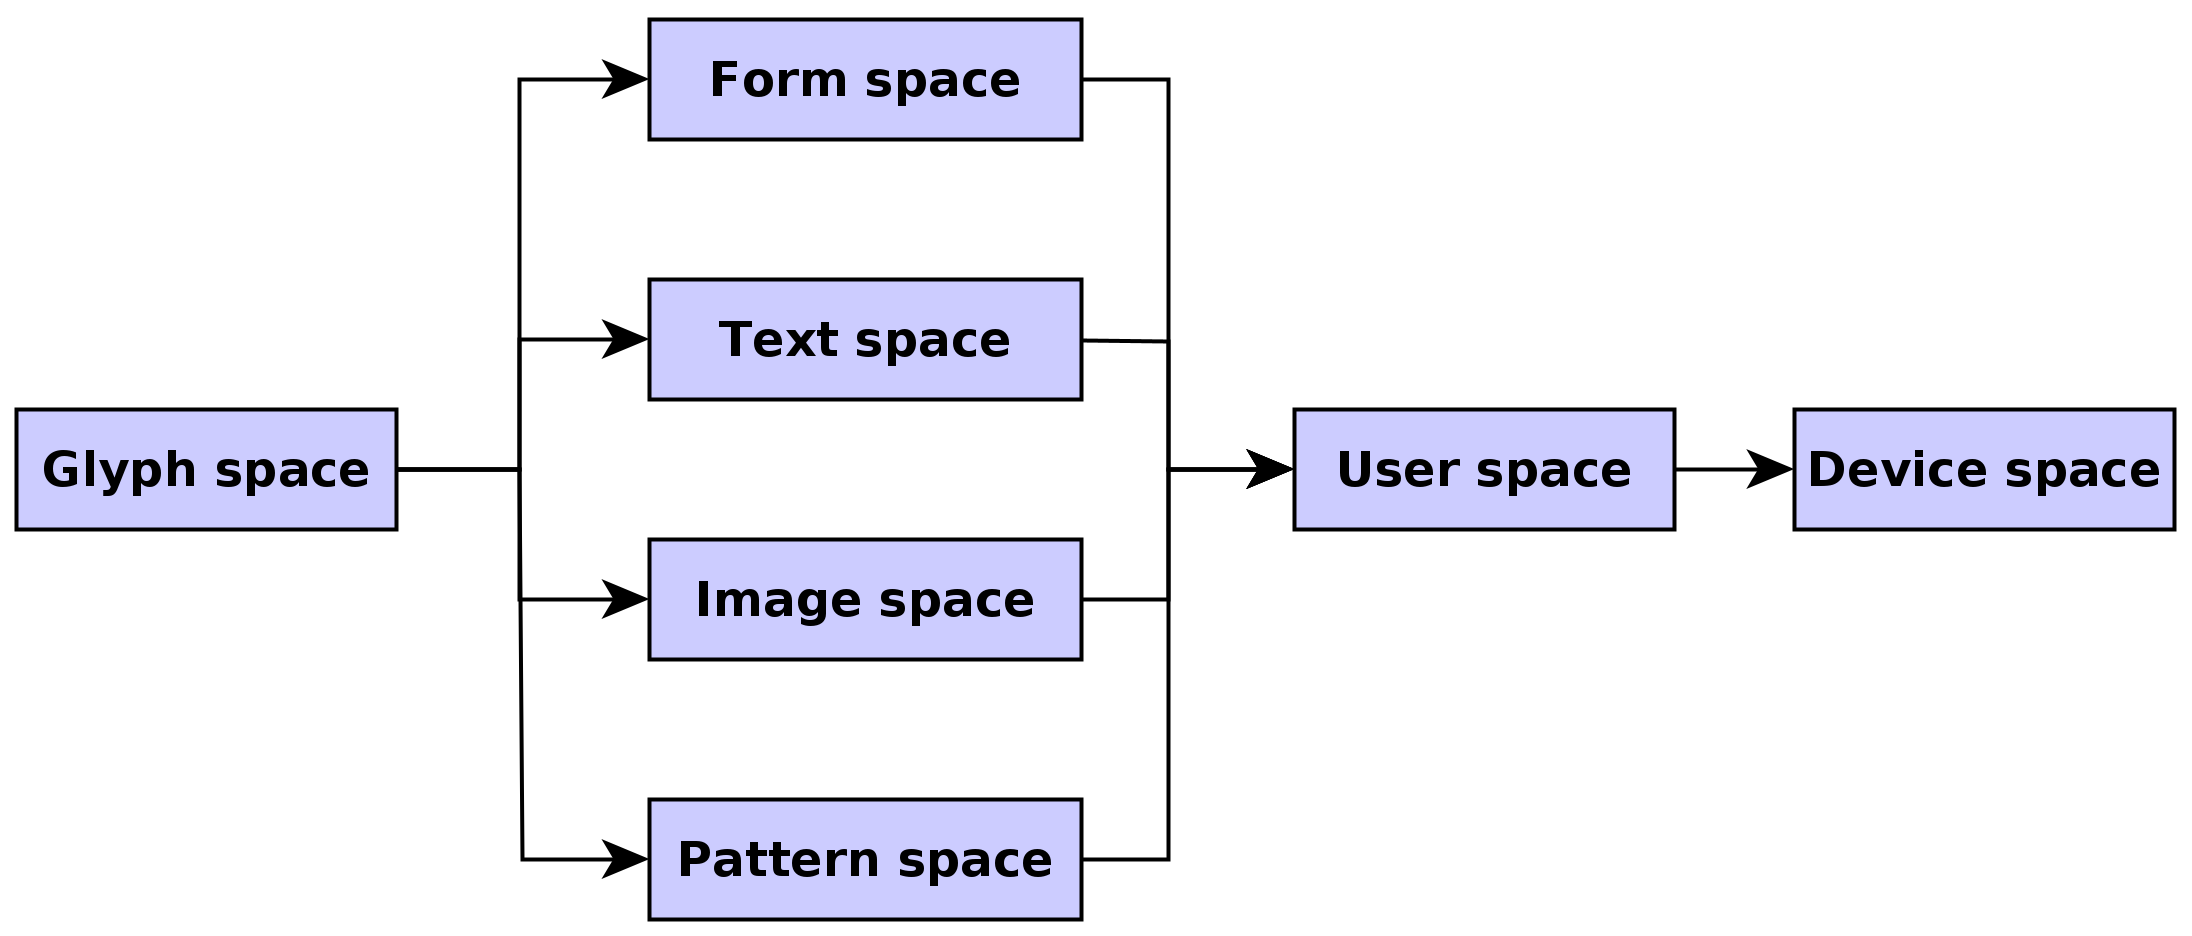
\includegraphics[width=11cm]{imaxes/espacios-coordenadas.png}
\end{figure}

¿Por qué el formato PDF almacena las coordenadas de las regiones?

\section{Información de coordenadas en documentos}
\subsection{El microformato HOCR y otras alternativas}
\subsection{Pdftotext e información de bounding box}

\section{OCR con Tesseract}
\section{Transformada de Hough}
\section{GNU Make}
\section{Flex y Bison}
\section{Ansible}
\section{Docker}


%% Valorar si mencionar otras herramientas como:
% Extracción de texto: Apache PDFBox, pdftotext
% OCR: Tesseract
% Pretty print de JSON: jq
